% Restructured book: content replaced from the supplied Chapter 2 DOCX.
\chapter{Requirement Survey and Analysis}
\newcommand{\ucflow}[1]{\begin{minipage}[t]{\linewidth}\begin{enumerate}[leftmargin=1.2em,nosep]#1\end{enumerate}\end{minipage}}

This chapter analyzes the requirements of RoomFlow as an AI-assisted interior design system. The overall goal is to transform a \textbf{user-provided design specification}, which includes a natural-language design brief and room geometry, into a \textbf{photorealistic interior design output}. To make this end-to-end problem controllable and editable, RoomFlow divides the process into two closely related sub-problems: \textbf{Automatic Interior Layout Design}, which generates a structured and editable furniture layout from the design specification, and \textbf{Layout-Guided Photorealistic Rendering}, which converts the selected 3D layout into a realistic image while preserving the spatial arrangement. Based on this perspective, the chapter reviews existing AI-based approaches for both sub-problems as well as for the overall end-to-end interior design task, and then derives the functional and non-functional requirements needed to develop RoomFlow.

\section{Survey of Existing Approaches}\label{sec:status-survey}

To derive concrete requirements for RoomFlow, this section reviews existing AI-based approaches related to the target problem. The survey first considers the overall end-to-end task of generating a photorealistic interior design output from a user-provided design specification, since this is the final result that RoomFlow aims to support. It then examines the two technical directions used by RoomFlow to make the task controllable and editable: Automatic Interior Layout Design and Layout-Guided Photorealistic Rendering. The section concludes by identifying the remaining gaps in existing approaches and translating them into requirements for RoomFlow.

\subsection{End-to-End AI-Assisted Interior Design}\label{subsec:integrated-layout-to-visualization-workflows}

End-to-end AI-assisted interior design aims to connect user requirements, design reasoning, spatial planning, layout optimization, and visual output within one workflow. This direction is broader than automatic furniture placement alone, because the system must preserve the user's design intent across several stages of the design process. It is also broader than photorealistic rendering alone, because the visual output should be grounded in a structured design state instead of being generated as an isolated image.

Recent works have explored this connected direction. Co-Layout uses an LLM-based workflow to extract room and furniture constraints from textual requirements, solves the resulting layout problem with grid-based integer programming, and converts the result into a 3D visualization with asset retrieval and rendering \cite{xiang2025colayout}. HOLODECK uses an LLM to decompose a prompt into floor plans, materials, doors, windows, object selection, and spatial constraints before arranging 3D assets in an interactive environment \cite{al2024HolodeckLanguageGuided}. These systems show that LLMs are useful for translating high-level user intent into structured design decisions, while optimization or rule-based modules are still needed for spatial plausibility.

For RoomFlow, the end-to-end requirement is more specific to interactive room design. The system must start from a user-provided design specification, generate an editable layout, preserve fixed room elements such as doors and windows, support 3D preview, and produce a layout-consistent photorealistic design output. Therefore, RoomFlow treats the editable layout as the central design state that connects automatic layout design, photorealistic rendering, and later image editing.

\subsection{Automatic Interior Layout Design}\label{subsec:ai-based-interior-layout-generation}

Automatic Interior Layout Design focuses on converting user-provided design specification into a structured furniture layout. The output is not a photorealistic image, but a representation of objects, sizes, positions, orientations, and spatial relations that can be checked, edited, and later visualized. This task is important because a useful interior design system must first decide what furniture should appear and where it should be placed before producing any realistic render.

Recent studies approach this task in different ways. LayoutGPT shows that an LLM can act as a visual planner and generate 2D or 3D layouts from text conditions \cite{al2023LayoutgptCompositionalVisual}. I-Design uses multiple LLM agents to transform user preferences into a scene graph, then applies a placement algorithm to obtain object positions \cite{al2024IDesignPersonalized}. FlairGPT uses structured LLM queries to extract zones, objects, attributes, and placement constraints, then solves the layout with constrained optimization \cite{Littlefair2025FlairgptRepurposingLlms}. LLplace further explores LLM-based 3D layout generation and editing through dialogue, while InstructScene uses a semantic graph prior and layout decoder to improve controllability in instruction-driven indoor scene synthesis \cite{yang2024llplace,lin2024instructscene}.

These works show that LLMs and graph-based representations are useful for interpreting design intent and producing structured layout plans. Their limitation is that semantic plausibility does not automatically guarantee geometric validity in a user-defined room. Layouts may still contain out-of-bound objects, overlaps, blocked openings, or weak circulation, especially when the room shape and fixed openings are important. RoomFlow therefore follows a hybrid direction: the language model is used for semantic planning, while room modeling, constraint checking, geometric solving, and final selection are handled by dedicated layout modules.

\subsection{Layout-Guided Photorealistic Rendering}\label{subsec:interior-image-generation-and-editing-survey}

Layout-Guided Photorealistic Rendering focuses on converting a given spatial layout into a realistic visual output while preserving the main room structure and furniture arrangement. This task is different from text-to-image generation, where the model may freely invent geometry from a prompt. In interior design, the visual result should remain consistent with the selected layout, including the room shell, openings, camera view, and major furniture positions.

Recent works address this problem by using layout or 3D structure as an explicit condition for appearance generation. Ctrl-Room separates text-to-3D room generation into a layout generation stage and an appearance generation stage, where the generated 3D layout is converted into a semantic layout map to guide panorama generation and panoramic NeRF reconstruction \cite{al2025CtrlRoomControllable}. SceneCraft converts 3D semantic layouts into multi-view 2D proxy maps and uses semantic- and depth-conditioned diffusion to generate multi-view images for learning a NeRF representation \cite{yang2024scenecraft}. SpatialGen further explores layout-guided 3D indoor scene generation by using a 3D layout and a reference image to synthesize realistic and semantically consistent indoor scenes from multiple viewpoints \cite{fang2025spatialgen}.

These works show that spatial conditioning is important for producing realistic interior images or scenes that remain faithful to a layout. However, many existing methods target full 3D scene or panorama generation and often require specialized training data, semantic layout maps, or reconstruction pipelines. RoomFlow follows a lighter application-oriented direction. It starts from the selected editable 3D layout, captures a camera-specific snapshot, combines it with visible-object metadata and preservation constraints, and uses this package to guide photorealistic rendering and later localized image editing. This keeps the rendered image connected to the editable layout instead of treating it as an independent generated image.

\subsection{General Assessment and Requirement Identification}\label{subsec:general-assessment-and-requirement-identification}

The surveyed approaches show that AI-assisted interior design cannot be handled reliably as a single free-form generation step. End-to-end systems demonstrate the value of connecting design reasoning, spatial planning, and visual output, but they still need stronger support for user control, editability, and traceability in an interactive room-design application. Automatic layout-design methods can transform user intent into structured furniture plans, but their outputs still need explicit room geometry, opening constraints, collision checks, and circulation validation. Layout-guided rendering methods can produce realistic visual results from spatial evidence, but the generated image may still drift from the selected layout if preservation constraints are not enforced.

These observations define the main requirements for RoomFlow. First, the system must store the room boundary, doors, and windows as explicit geometric data rather than relying on text alone. Second, semantic design reasoning and geometric placement must be separated: the language model should interpret the user's design intent, while dedicated geometric modules should solve and validate object placement. Third, the generated layout must remain editable, with furniture identities, dimensions, positions, and orientations preserved as structured data. Fourth, photorealistic rendering must be derived from the selected 3D layout through a snapshot, visible-object metadata, and preservation constraints, so that the image remains connected to the editable design state. Finally, localized image editing must keep a traceable link to the source render, target region, and original layout, reducing unintended changes to unrelated parts of the room.

\section{Functional Overview}\label{sec:functional-overview}

After deriving the main requirements in Section 2.1, this section presents RoomFlow from a functional perspective. The purpose is to describe the high-level functions that support the early-stage interior design workflow, before the detailed use case specifications are given in Section 2.3. The workflow starts from room creation and design input, continues with automatic layout generation and manual layout editing, and then proceeds to 3D preview, layout-guided photorealistic rendering, localized image editing, and result management.

The core user workflow is organized around the two technical sub-problems of RoomFlow. For \textbf{Automatic Interior Layout Design}, the system allows the user to define a room, specify fixed openings, provide a design brief, generate layout variants, and revise the selected layout in an editable workspace. For \textbf{Layout-Guided Photorealistic Rendering}, the system converts the selected layout into a 3D preview, captures the chosen camera view, generates a realistic perspective render, and supports localized editing of the generated render while preserving unrelated room structure.

The use case model contains three human actors. A \textbf{Guest} can access the system and authenticate into an account. A \textbf{User} performs the main design workflow, including room creation, layout editing, automatic layout generation, 3D preview, render generation, image editing, and artifact management. An \textbf{Admin} maintains shared system data such as user accounts and furniture records. External AI services are treated as backend-supported components rather than human actors because they do not initiate user goals in the application.

\subsection{Main Use Case Model}\label{subsec:main-use-case-model}

\hyperref[fig:2-1]{Figure~2.1} presents the main use case model of the RoomFlow application. The diagram shows the system boundary, the three human actors, and the principal functions available to each actor.

\begin{figure}[!htbp]
\centering
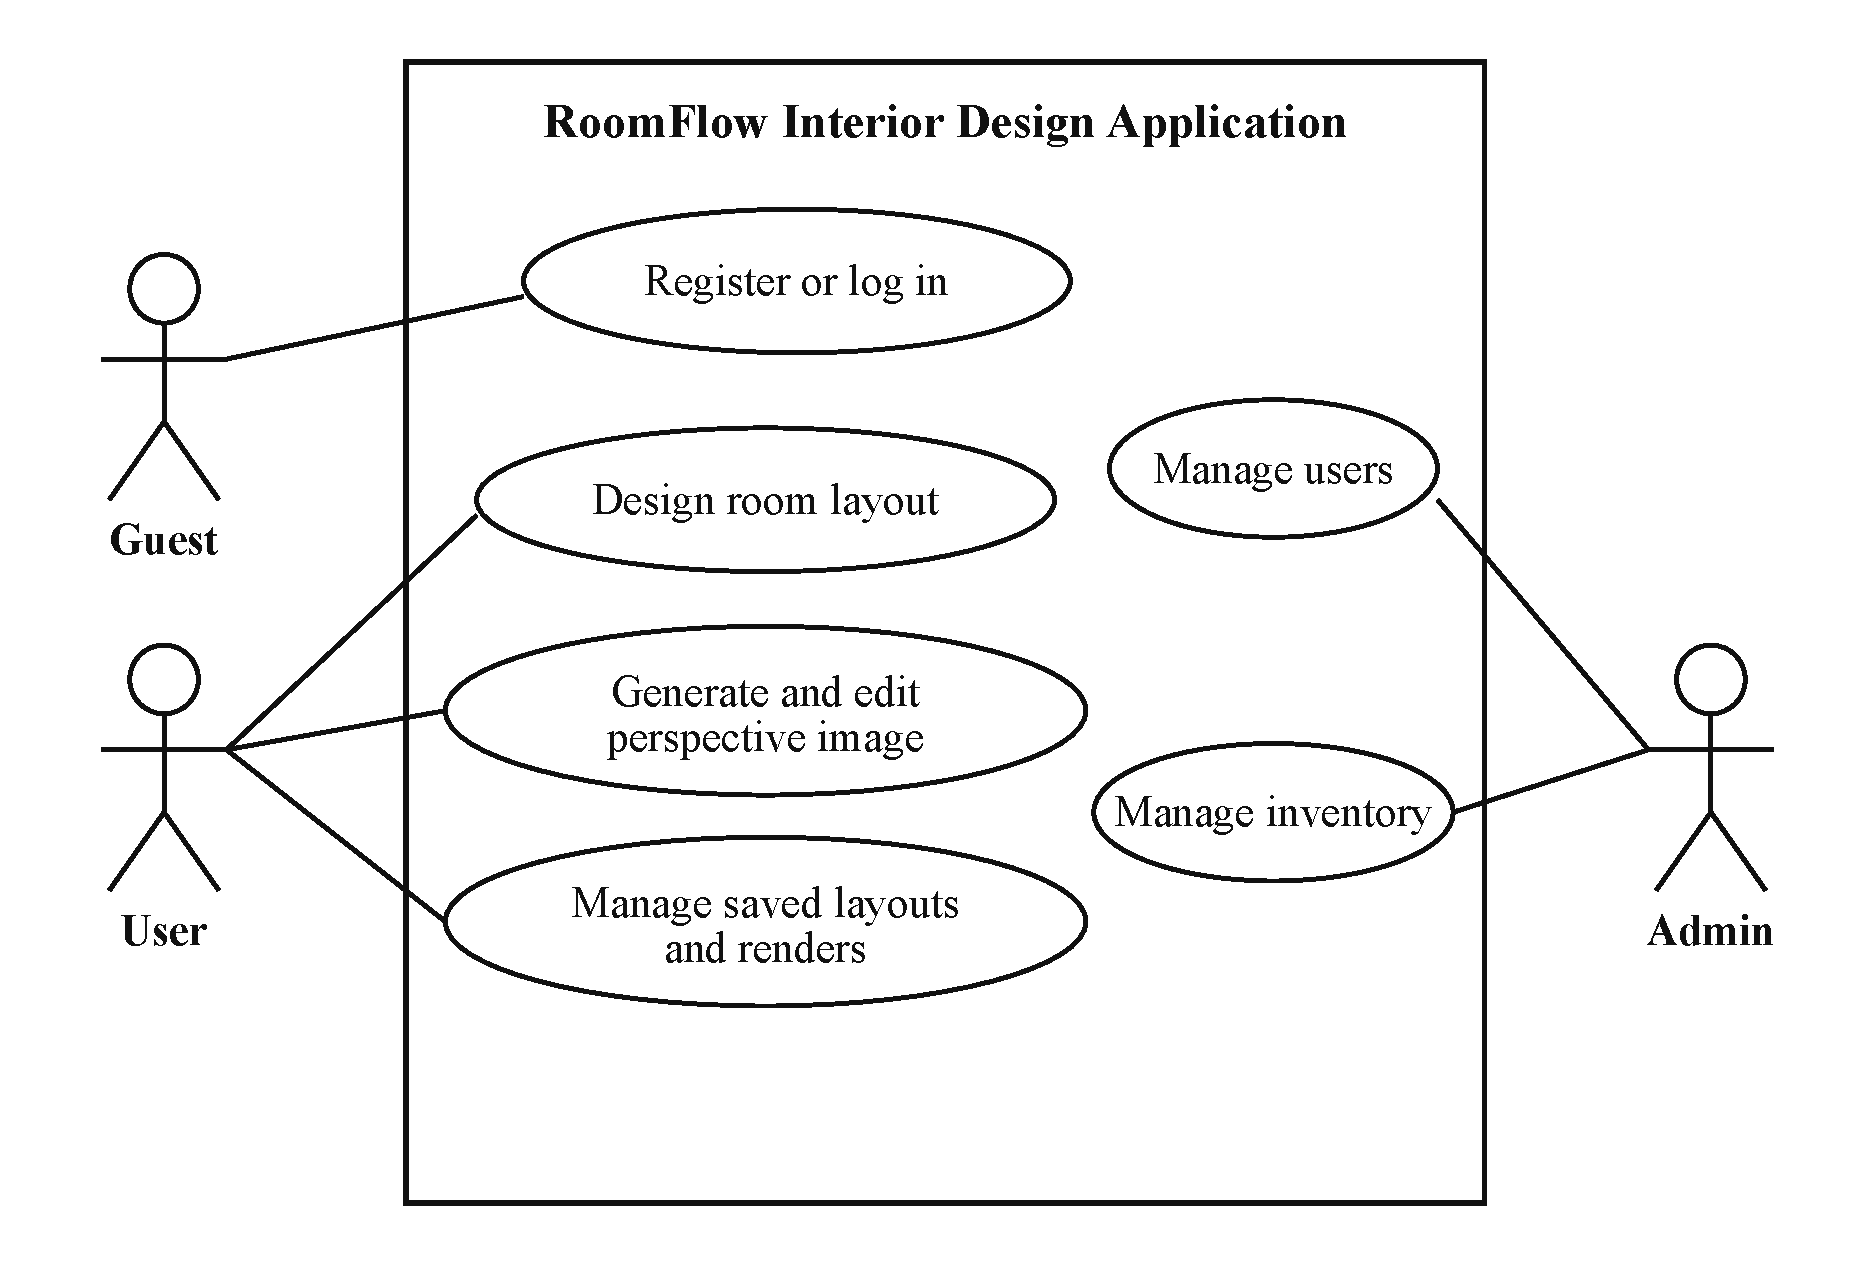
\includegraphics[width=0.94\textwidth]{figures/chapter2/figure_01.pdf}
\caption{Main use case model of the RoomFlow application.}
\label{fig:2-1}
\end{figure}

The Guest actor can register and log in. After authentication, the User can create a room, manually design a room layout, automatically generate a room layout, generate a 3D preview, generate a perspective image, edit a perspective image, and save or load layout and render artifacts. The Admin actor can add users, deactivate users, and add furniture records to the inventory.

The model emphasizes that RoomFlow is not only an image-generation tool. It starts from room geometry, creates editable layout data, and uses that layout as the source for 3D preview and perspective rendering. The detailed specifications later in this chapter are limited to the three use cases most directly related to the thesis contributions.

\subsection{Detailed Use Case Diagrams for Core Workflows}\label{subsec:decomposed-use-case-diagram}

This section provides separate detailed diagrams for the two core use cases studied in this thesis. The first use case supports automatic editable layout generation. The second use case supports layout-consistent perspective rendering from the selected layout. Each diagram follows the same simple use-case style as \hyperref[fig:2-1]{Figure~2.1}: actor, system boundary, and the main user-visible sub-use cases.

Figure~\ref{fig:2-2} decomposes the Auto Design Room Layout workflow into the user-visible actions needed before and after automatic generation. Figure~\ref{fig:2-3} decomposes the Generate Perspective Image workflow, where the user selects a layout, previews it in 3D, chooses camera and preset settings, and saves the resulting render.

\begin{figure}[!htbp]
\centering
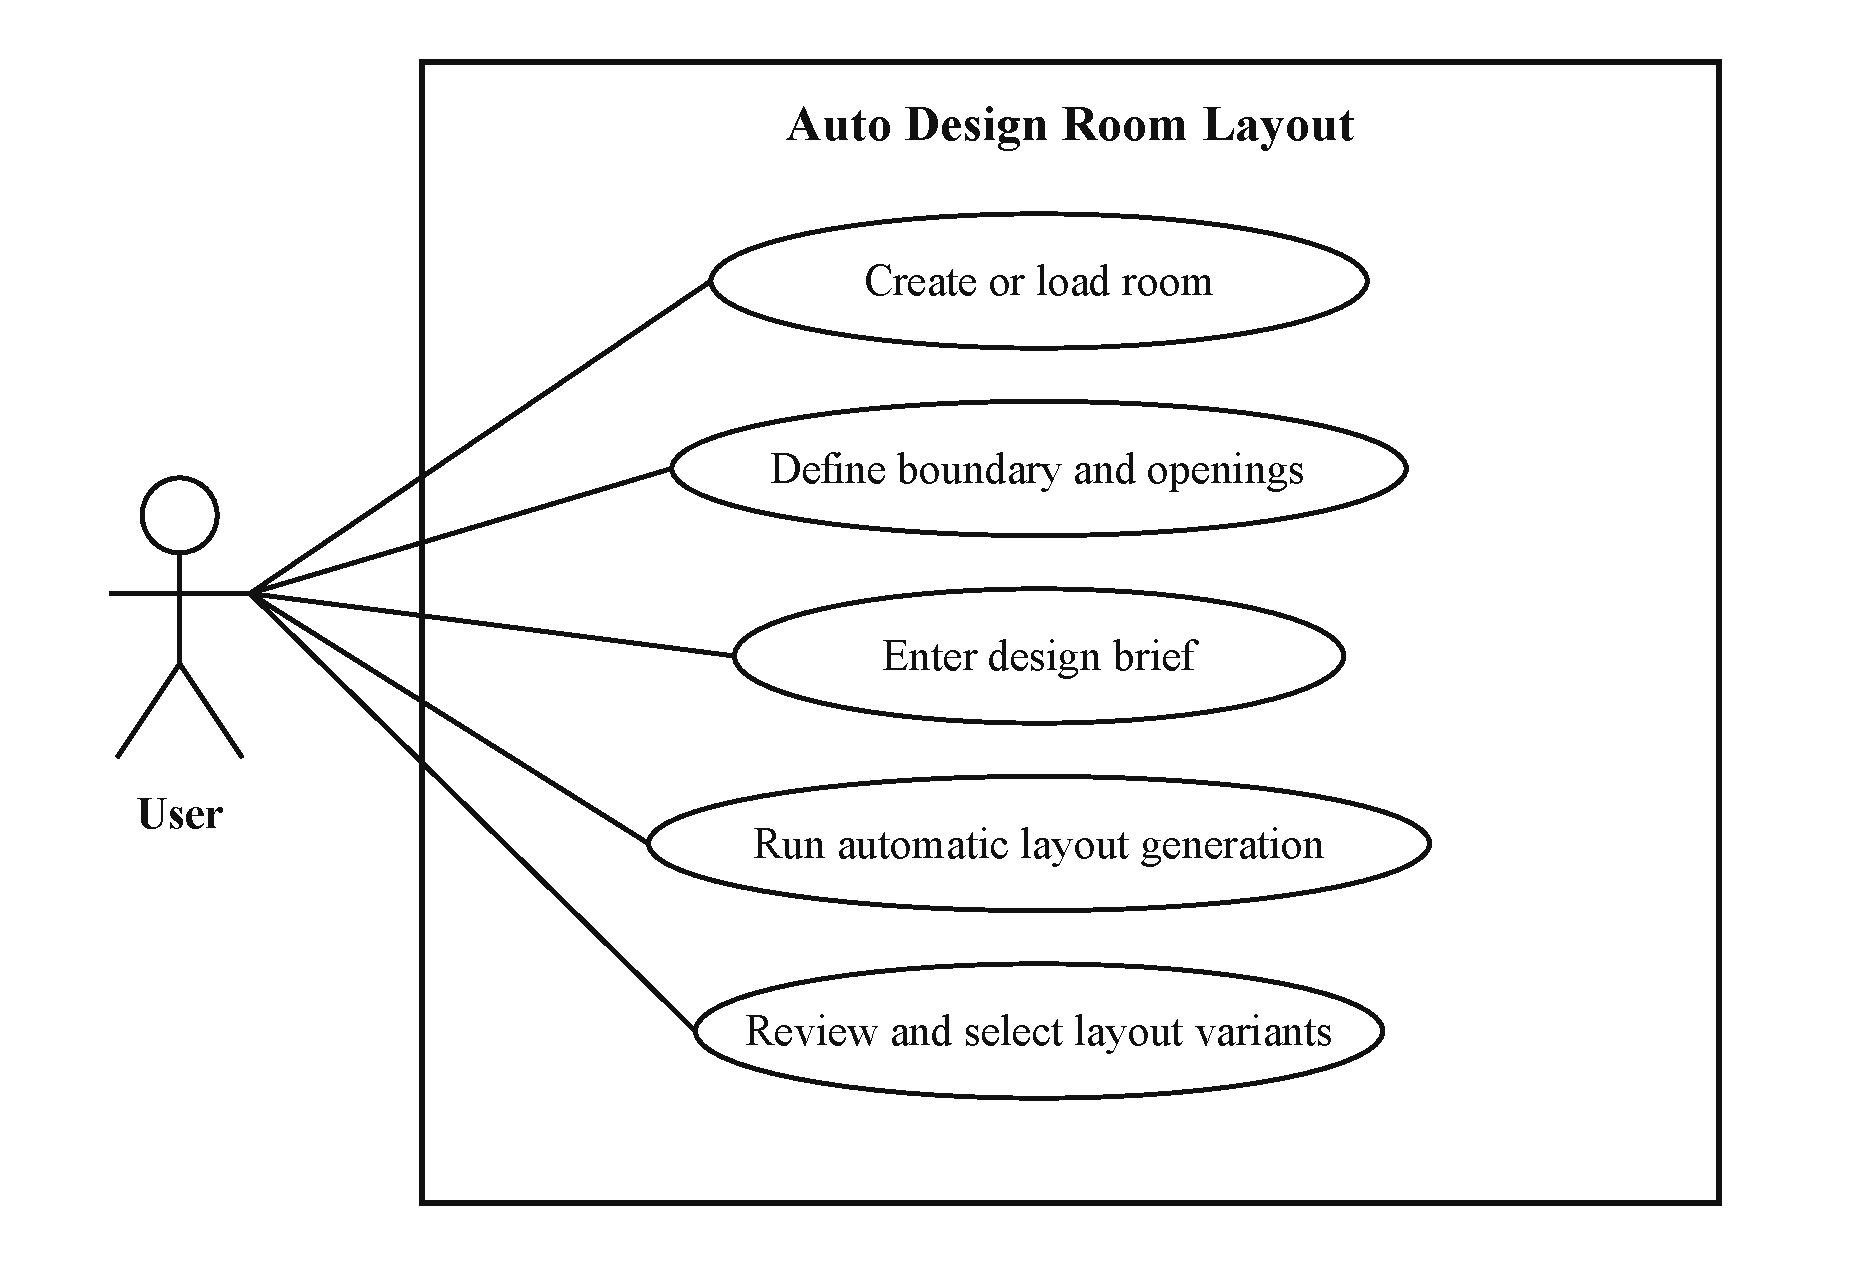
\includegraphics[width=0.94\textwidth]{figures/chapter2/figure_02_auto_design_room_layout.pdf}
\caption{Detailed use case diagram for Auto Design Room Layout.}
\label{fig:2-2}
\end{figure}

\begin{figure}[!htbp]
\centering
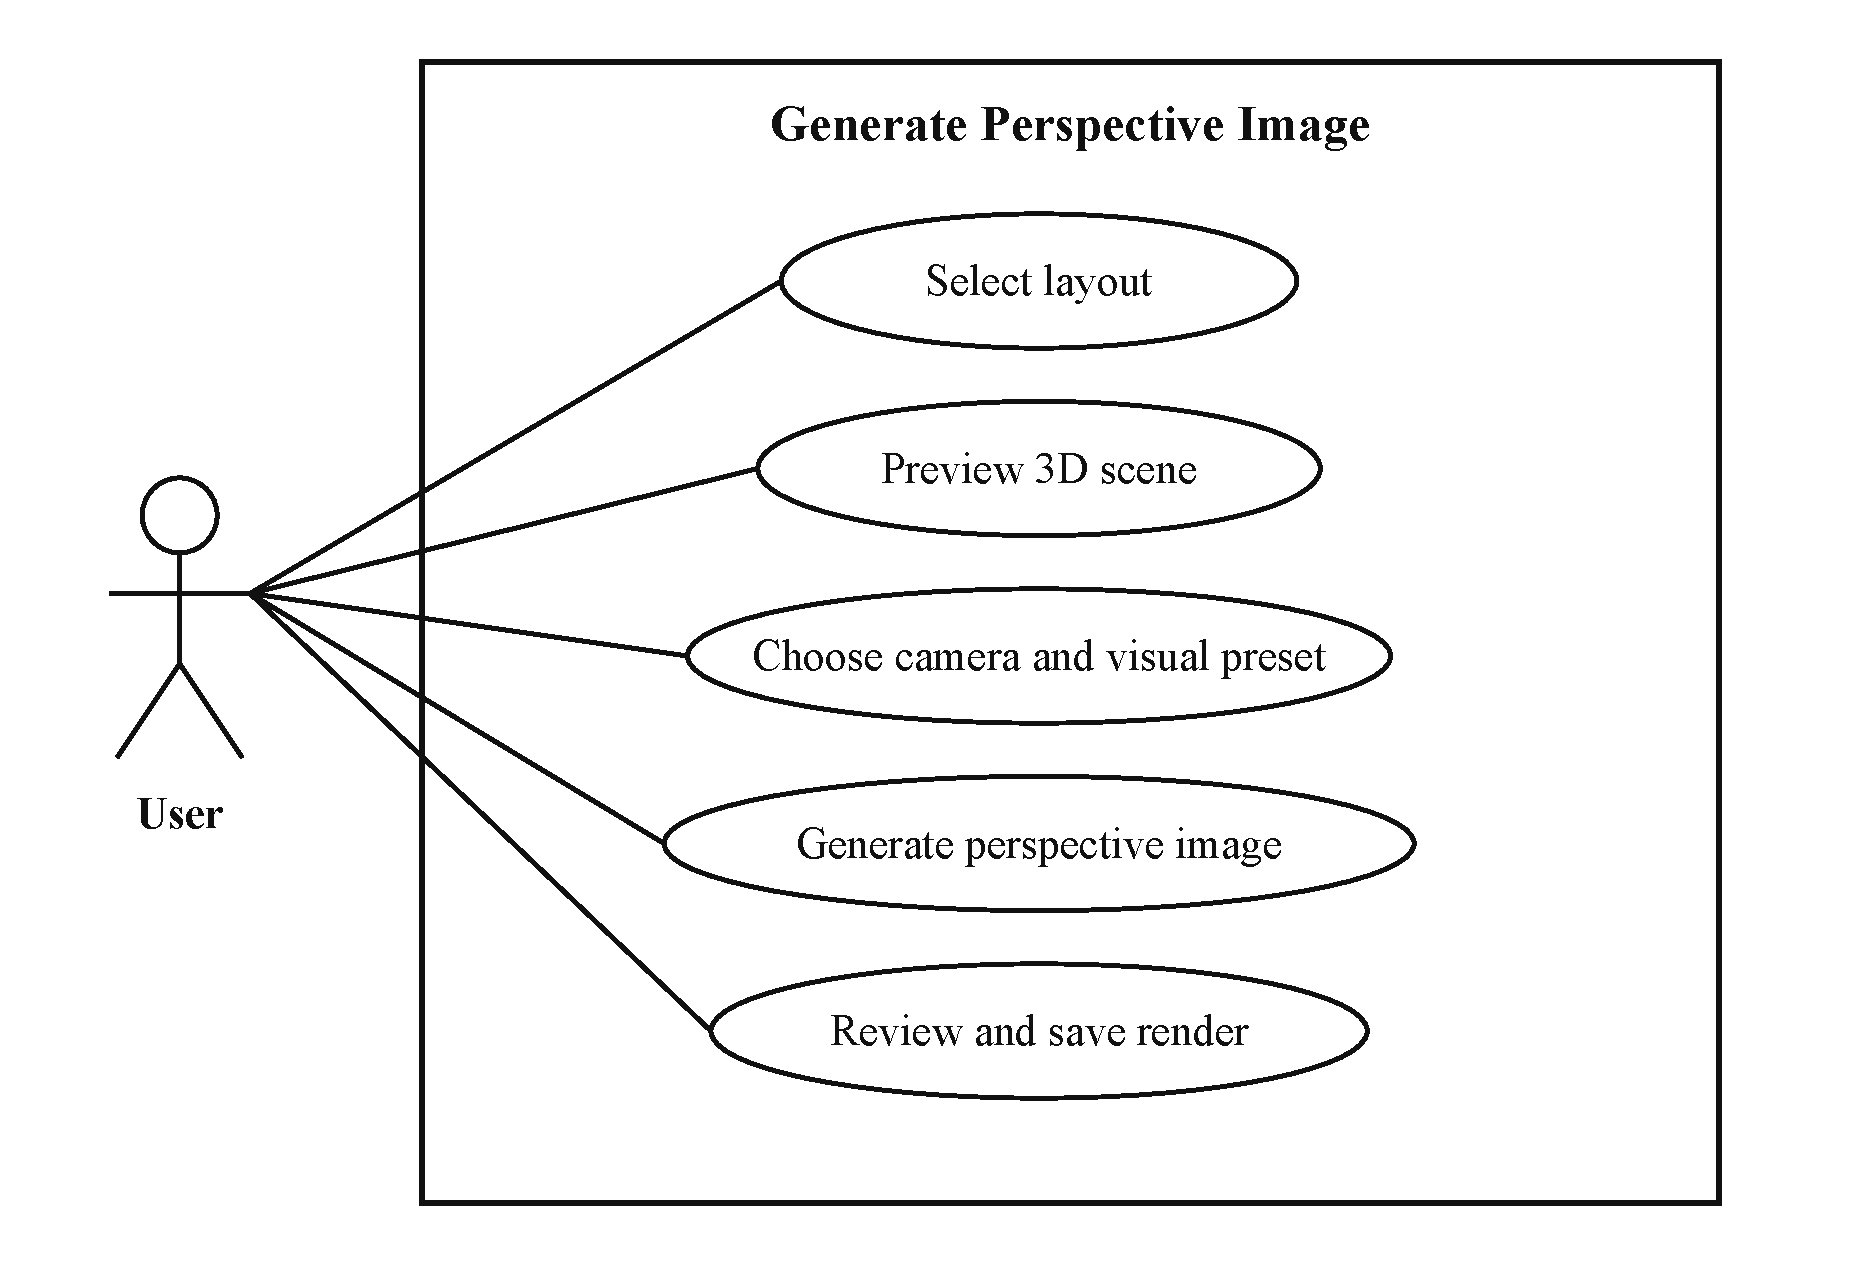
\includegraphics[width=0.94\textwidth]{figures/chapter2/figure_03_generate_perspective_image.pdf}
\caption{Detailed use case diagram for Generate Perspective Image.}
\label{fig:2-3}
\end{figure}

\subsection{Business Process for Layout Design and Visualization}\label{subsec:business-process-layout-design-visualization}

\begin{figure}[!htbp]
\centering
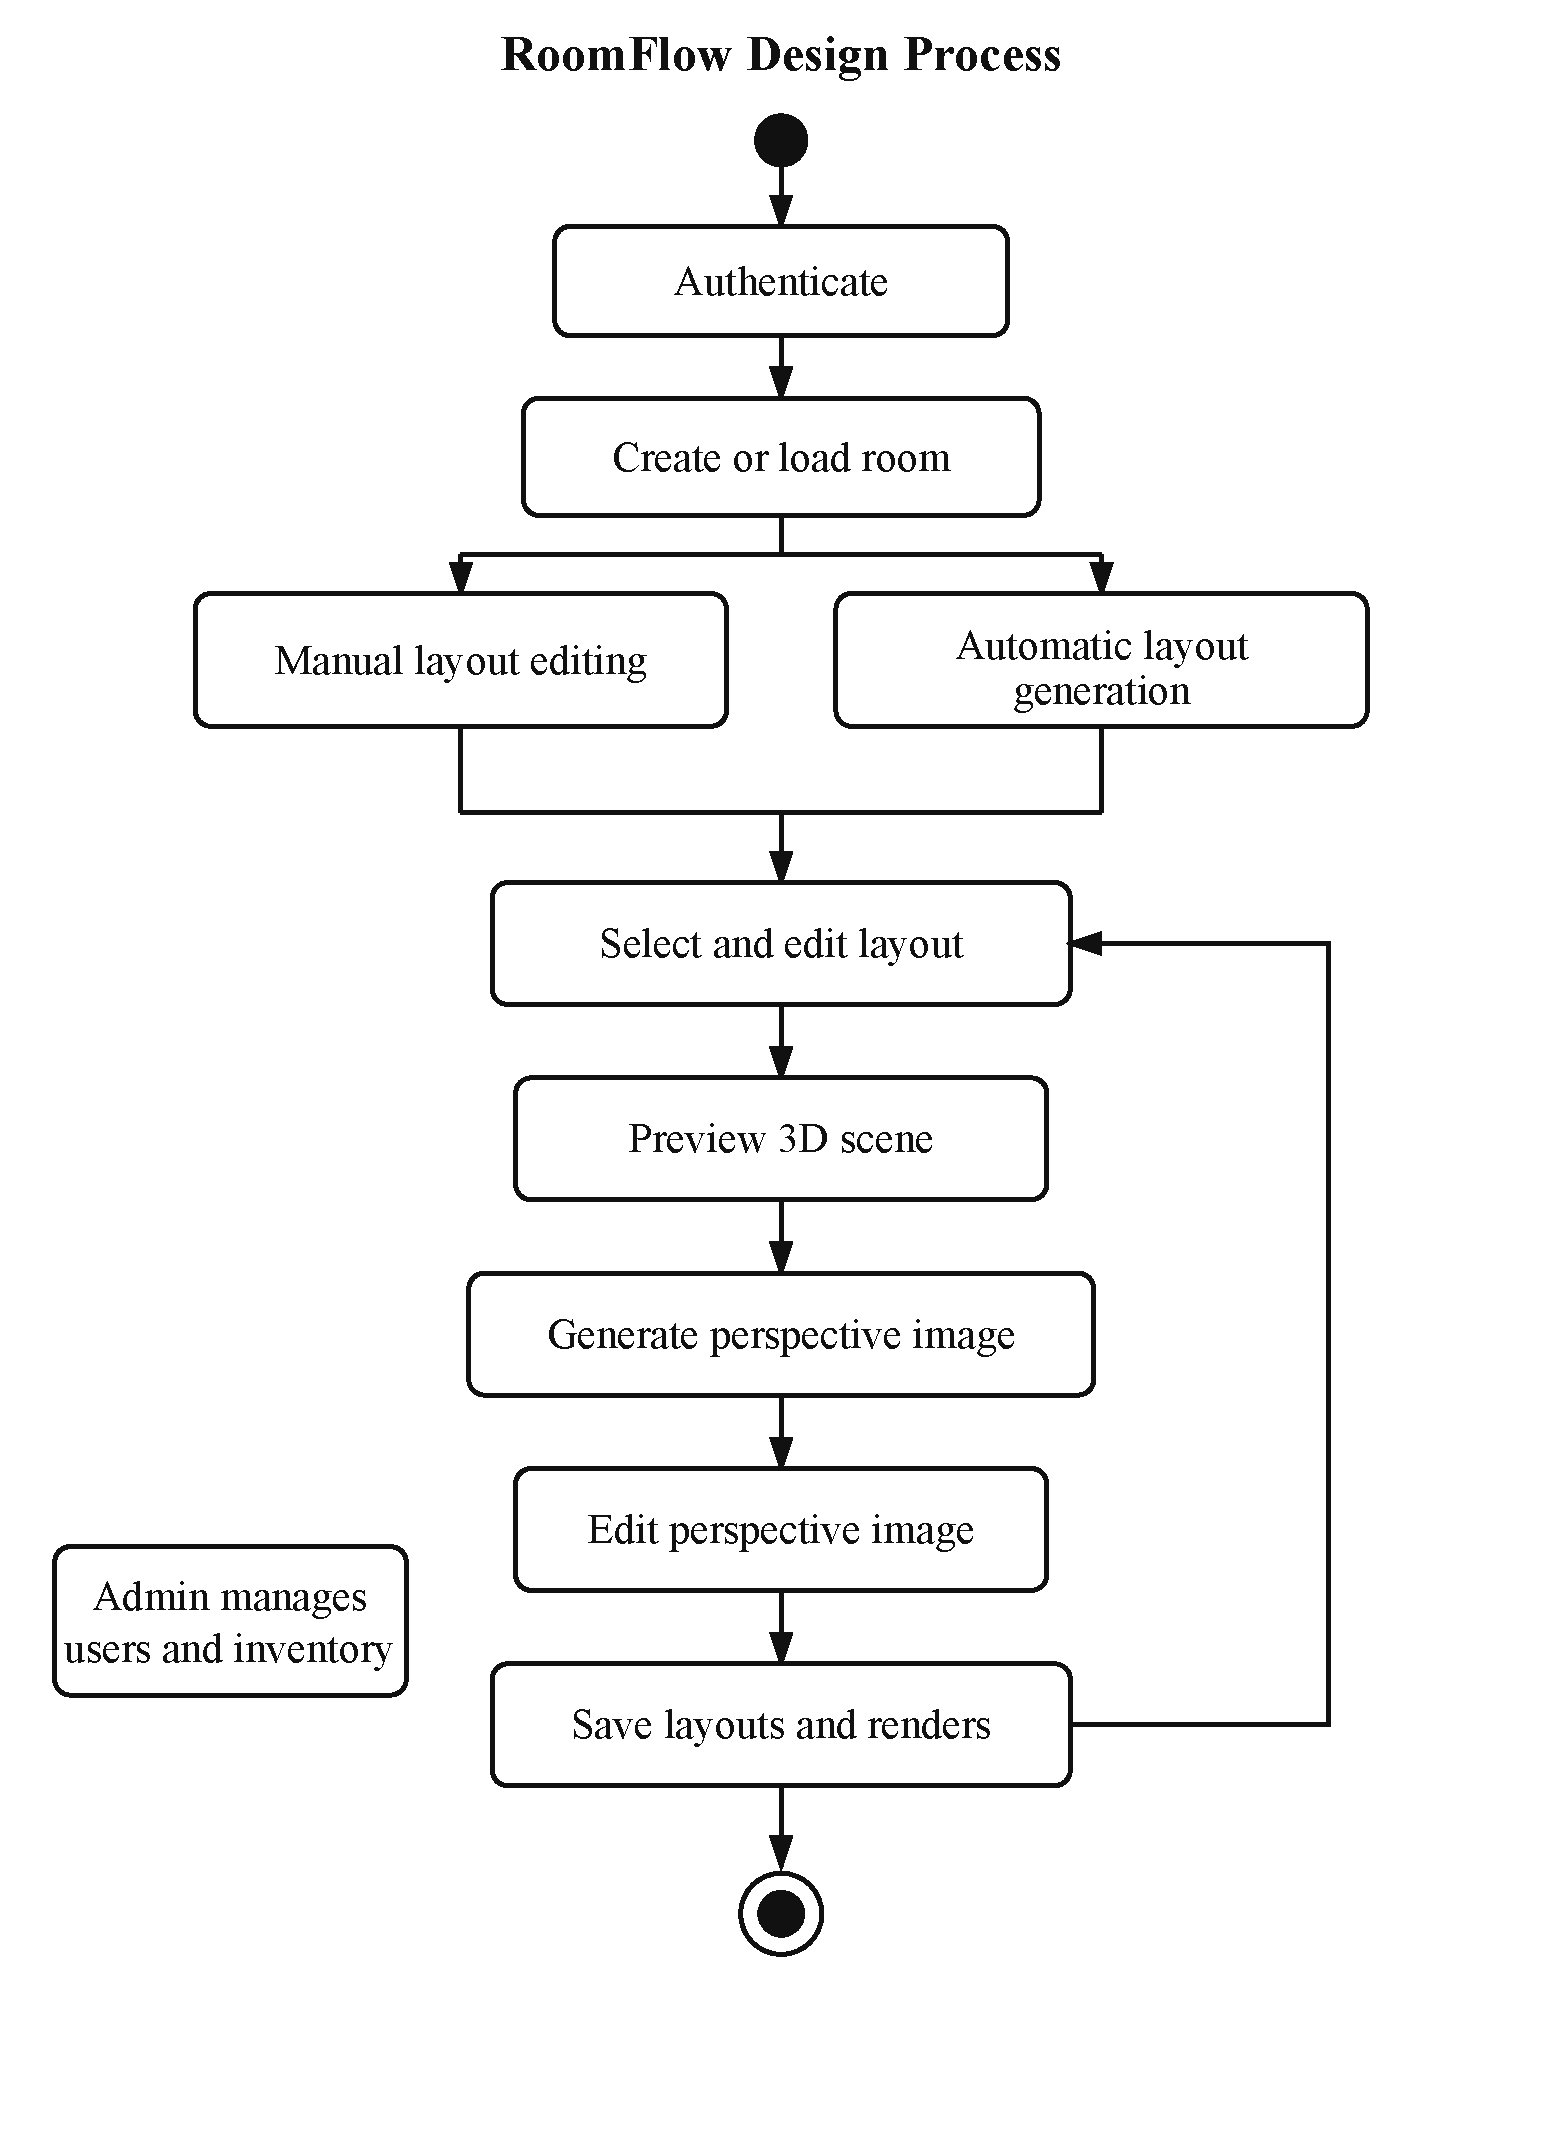
\includegraphics[width=0.82\textwidth]{figures/chapter2/figure_07.pdf}
\caption{Business process for AI-assisted interior design in RoomFlow.}
\label{fig:2-4}
\end{figure}

Figure~\ref{fig:2-4} presents the main workflow of the system. After logging in, the user starts a design session by creating a new room or loading a saved room. A room contains the basic information required for later processing, including the room type, boundary, doors, windows, and design brief.

The design flow then continues through two possible layout paths. In the manual path, the user directly arranges furniture in the 2D workspace. In the automatic path, the system uses the room data, design brief, and furniture inventory to generate editable layout variants. The user reviews these variants, selects one layout, and may continue adjusting it manually. This loop keeps the automatic result as a starting point while preserving user control over the final arrangement.

After the layout is accepted, the system converts it into a 3D preview. From the selected camera view, the user can generate a perspective render image. If the render needs further refinement, the user can either return to layout editing and render again, or request a localized image edit on the existing render. The workflow ends when the user saves the layout, render, or edited render for later reuse.

The revision loop in Figure~\ref{fig:2-4} highlights that rendering is not a separate one-way step: if the generated perspective image reveals a layout issue, the user can return to the editable layout before generating a new visualization.

Admin management is outside the main design flow. It maintains user accounts and furniture records so that the design workflow can operate with valid users and consistent inventory data.

\section{Functional Description}\label{sec:functional-description}

This section specifies the three use cases most closely connected to the thesis contributions. Authentication, room creation, manual editing, saved-artifact management, and administrator functions remain visible in Figure~\ref{fig:2-1}, but they are conventional supporting functions and are not expanded into separate specifications. Tables~\ref{tab:2-3}, \ref{tab:2-4}, and \ref{tab:2-5} focus on automatic layout design, perspective-image generation, and localized image editing.

\subsection{Use Case UC01: Auto Design Room Layout}\label{subsec:uc01-auto-design-room-layout}

\begingroup
\small
\setlength{\tabcolsep}{5pt}
\renewcommand{\arraystretch}{1.15}
\begin{xltabular}{\textwidth}{|>{\raggedright\arraybackslash}p{3.1cm}|>{\raggedright\arraybackslash}X|}
\caption{Use case specification for Auto design room layout.}\label{tab:2-3}\\
\hline
\textbf{Item} & \textbf{Description} \\
\hline
Use case ID & UC01 \\
\hline
Use case name & Auto design room layout \\
\hline
Description & The system generates editable furniture layout variants from the user brief, room geometry, openings, and furniture inventory. \\
\hline
Actor & User \\
\hline
Precondition & A valid room has been created, fixed openings are available, and the user has entered a design brief. \\
\hline
Main flow & \ucflow{\item The user requests automatic layout generation. \item The system sends the room geometry, openings, brief, and inventory scope to the backend pipeline. \item The semantic planning stage extracts required objects, optional objects, style intent, and object relations. \item The room modeling stage derives geometric constraints from the room boundary and openings. \item The solver generates candidate layouts and checks spatial constraints. \item The system returns multiple layout variants with diagnostics. \item The user reviews the variants and selects one as the working layout.} \\
\hline
Alternative flow & If no valid layout is found, the system reports the issue and suggests reducing furniture requirements, changing the room input, or editing manually. \\
\hline
Postcondition & One or more editable layout variants are available for manual refinement, 3D preview, and rendering. \\
\hline
\end{xltabular}
\endgroup

This use case connects natural-language design requirements with explicit geometric validation so that the output is not only plausible but also usable as an editable room layout.

\subsection{Use Case UC02: Generate Perspective Image}\label{subsec:uc02-generate-perspective-image}

\begingroup
\small
\setlength{\tabcolsep}{5pt}
\renewcommand{\arraystretch}{1.15}
\begin{xltabular}{\textwidth}{|>{\raggedright\arraybackslash}p{3.1cm}|>{\raggedright\arraybackslash}X|}
\caption{Use case specification for generating a perspective image.}\label{tab:2-4}\\
\hline
\textbf{Item} & \textbf{Description} \\
\hline
Use case ID & UC02 \\
\hline
Use case name & Generate 3D preview and perspective image \\
\hline
Description & The user opens the 3D preview of a selected editable layout, chooses a camera view, and asks the system to generate a perspective render from that view. \\
\hline
Actor & User \\
\hline
Precondition & A valid layout has been selected and a 3D preview can be generated. \\
\hline
Main flow & \ucflow{\item The user opens the 3D preview of the selected layout. \item The frontend reconstructs the room shell, openings, and furniture from the editable layout. \item The user chooses or adjusts a camera view. \item The system captures a 3D snapshot and layout metadata. \item The system compiles a prompt package containing room structure, visible objects, style preset, lighting preset, and preservation constraints. \item The image-generation provider returns a perspective render. \item The system stores the render with a link to the source layout.} \\
\hline
Alternative flow & If image generation fails, the system reports the failure and allows the user to retry or adjust the input. \\
\hline
Postcondition & A perspective render image is generated and remains traceable to the selected layout. \\
\hline
\end{xltabular}
\endgroup

The 3D preview is a required step because the perspective image is derived from its selected camera view and snapshot. The generated render remains a visual layer linked to the editable layout rather than becoming the primary design state.

\subsection{Use Case UC03: Edit Perspective Image}\label{subsec:uc03-edit-perspective-image}

\begingroup
\small
\setlength{\tabcolsep}{5pt}
\renewcommand{\arraystretch}{1.15}
\begin{xltabular}{\textwidth}{|>{\raggedright\arraybackslash}p{3.1cm}|>{\raggedright\arraybackslash}X|}
\caption{Use case specification for Edit perspective image.}\label{tab:2-5}\\
\hline
\textbf{Item} & \textbf{Description} \\
\hline
Use case ID & UC03 \\
\hline
Use case name & Edit perspective image \\
\hline
Description & The user requests a localized edit on a generated render image. \\
\hline
Actor & User \\
\hline
Precondition & A source render exists and is linked to a layout or selected image state. \\
\hline
Main flow & \ucflow{\item The user selects an edit operation, such as add, remove, replace, or recolor. \item The user selects the target object or target region when available. \item The system prepares the source render, target scope, operation instruction, and preservation constraints. \item The image-editing provider returns an edited image. \item The system stores the edited image and links it to the source render.} \\
\hline
Alternative flow & If the target object or region cannot be identified, the system asks the user to refine the target selection or use a more general edit instruction. \\
\hline
Postcondition & An edited render is produced while preserving unrelated room structure as much as possible. \\
\hline
\end{xltabular}
\endgroup

This use case keeps visualization interactive. The user does not need to restart the complete workflow when only a local visual change is needed.

\section{Non-Functional Requirements}\label{sec:non-functional-requirements}

Besides functional requirements, the system must satisfy several non-functional requirements. These requirements are important because the application combines interactive editing, AI generation, geometric validation, image rendering, and persistent user data.

Table~\ref{tab:2-6} summarizes the non-functional requirements used to guide the system design and later implementation choices.

\begingroup
\small
\setlength{\tabcolsep}{4pt}
\renewcommand{\arraystretch}{1.15}
\begin{xltabular}{\textwidth}{|>{\raggedright\arraybackslash}p{1.6cm}|>{\raggedright\arraybackslash}p{3.1cm}|>{\raggedright\arraybackslash}X|}
\caption{Non-functional requirements.}\label{tab:2-6}\\
\hline
\textbf{ID} & \textbf{Requirement} & \textbf{Description} \\
\hline
NFR-01 & Usability & The interface should be understandable for non-professional users and should not require specialized drafting knowledge or interior-design terminology. Common actions should be available through visible controls rather than raw JSON editing. \\
\hline
NFR-02 & Editability & Generated layouts must remain editable after automatic generation. The system should not treat AI output as a fixed final result. \\
\hline
NFR-03 & Spatial consistency & Layout generation should preserve room geometry, fixed openings, furniture dimensions, collision avoidance, and basic circulation. \\
\hline
NFR-04 & Visualization consistency & Rendered images should preserve the main room structure, camera view, openings, and major furniture arrangement from the selected layout. \\
\hline
NFR-05 & Reliability & The system should handle invalid room geometry, failed AI requests, missing furniture assets, and rendering failures without crashing the whole application. Long-running AI calls should expose progress and a clear failure message; retry should be possible when the provider or network fails. \\
\hline
NFR-06 & Maintainability & The system should separate frontend interaction, backend processing, solver logic, inventory data, persistence, and AI-provider integration. \\
\hline
NFR-07 & Security & Authentication data must be protected, raw tokens and passwords must not be logged, and administrator functions must be restricted to users with admin permission. \\
\hline
NFR-08 & Performance & Manual editing should feel immediate in the browser. As a design target, ordinary drag, rotate, and selection operations should update the 2D workspace within about 100 ms on typical laptop hardware. Long-running layout-generation and image-generation tasks may take longer, but the system should report progress within a few seconds and provide a clear retry path if the provider or network fails. \\
\hline
NFR-09 & Traceability & Generated layouts, renders, and edited renders should be linked to their source room, selected layout, prompt package, and relevant metadata. \\
\hline
NFR-10 & Cost control & Since AI generation may use external services, the system should avoid unnecessary repeated calls and reuse stored artifacts when possible. \\
\hline
\end{xltabular}
\endgroup

Usability and editability are the most important user-facing requirements. The target users are not professional designers, so they must be able to create a room, request a layout, adjust the result, and generate a render through direct interaction.

Spatial consistency and visualization consistency are the most important technical requirements. The system should not only produce visually pleasing outputs. It must preserve the design structure that the user created or selected. This requirement connects directly to the two problems introduced in Chapter 1.

Reliability, maintainability, traceability, and cost control are necessary because the system uses multiple AI and geometry-processing stages. Saving intermediate artifacts and separating modules make the system easier to debug, evaluate, and extend.
